\def\SigleNumero{STT-2902}
\def\NomCours{Modélisation statistique}
\def\DateEvaluation{6 octobre 2025}
\def\HeureEvaluation{8 h 30 à 10 h 20}
\def\Session{}
\def\NomEvaluation{Examen 1}
\def\Ponderation{}
% Ne rien mettre entre les accolades si l'enseignant (ou l'enseignante) est aussi le coordonnateur (ou la coordonnatrice)
\def\Coordonnatrice{}
\def\Coordonnateur{}

% Ne rien mettre entre les accolades s'il y a plus d'une section
\def\Enseignant{Julien Miron}
\def\Enseignante{}

% Ne rien mettre entre les accolades s'il s'agit d'un cours à section unique
% Mettre le nom de chacun des enseignants et enseignantes entre les accolades
% Une case à cocher sera générée pour chacune des sections
\def\SectionA{}
\def\SectionB{}
\def\SectionC{}
\def\SectionD{}


\def\Directives{
\begin{enumerate}
\item Matériel autorisé:
\begin{itemize}
    \item Calculatrice scientifique {\bf autorisée par la faculté des sciences et de génie};
    \item Votre cahier de notes de cours;
    \end{itemize}
\item Assurez-vous que cette évaluation comporte \numquestions ~questions réparties sur \numpages{}~pages, pour un total de \numpoints{}~points.\
\item \textbf{Veuillez ne pas dégrafer votre examen.}
\item Ajoutez vos initiales dans le bas de chaque page.
\item Vous devez\textbf{ justifier toutes vos réponses} par une démarche claire, sauf pour les questions à choix de réponse.\
\item Pour les questions à choix de réponse et les vrais ou faux, vous pouvez mettre un X, un crochet ($\checkmark$) ou remplir la case.\
\item Certains vrais ou faux demandent une justification. Aucun point ne sera donné sans justification, même si vous cochez la bonne réponse.
\item Pour les questions à choix de réponse, lorsqu'il est écrit «cochez tous les énoncés qui sont vrais/faux», il est possible qu'un seul énoncé soit vrai.
\item Le verso des feuilles peut être utilisé comme brouillon, \textbf{mais ne sera pas corrigé}. Attention à ne rien dégrafer.
\end{enumerate}
}



\documentclass{Examens/Evaluation}
\usepackage{multicol,graphicx}
\begin{document}

\pageblanche
%%%%%%%%%%%%%%%% QUESTION %%%%%%%%%%%%%%%%
\begin{questions}
\question\label{main}

Vous aimeriez connaître la consommation moyenne de boissons énergisantes par les étudiants de l'Université Laval en interrogeant \textbf{200 étudiants}.
En contactant le bureau du registraire (et en étant très convaincant), vous réussissez à obtenir ce tableau pour les 40\,000 étudiants inscrits au baccalauréat, à la maîtrise ou au doctorat à l'automne 2025:

\begin{table}[h]
    \centering
    \begin{tabular}{|c|c|c|c|c|c|c|}
    \hline
        Matricule\tablefootnote{Les matricules vont de 1 à 40\,000.} & Nom, Prénom & Faculté & Département & Programme & Moyenne cumulative\tablefootnote{La moyenne cumulative va de 0 à 4,33.}\\
        \hline
        1 & Nicosia, Aurélien & FSG & DMS & Ph.D. en statistique &4,33\\
        \hline 
        2 & Soucy, Jérôme & FSG & DMS & M.Sc. en mathématiques &2,72\\
        \hline
        3 & Bachand, Alex & FSA & CPT & B.Sc. en gestion Excel & 3,24\\
        \hline
        4 & Guérin, Amandine & MUS & PIA & Ph.D. en piano & 4,33 \\
        \hline
        5 & Bilodeau, Catherine & MED & RFX & Ph.D. en réflexologie & 4,21 \\
        \hline
... & ... & ... & ... & ... & ...\\
\hline
    \end{tabular}
    
\end{table}


\begin{parts}
    \part[3] Expliquez précisément comment vous devriez procéder pour utiliser un échantillon par grappes.

    

    \vspace{5cm}
    En étudiant le tableau, vous constatez qu'il existe 20 facultés qui ont toutes 10 départements. Chaque département a 10 programmes de 20 étudiants.\footnote{Bien sûr, ces chiffres sont fictifs, ils sont choisis car ils sont plus faciles à utiliser.}
    
    \part[5] Vous voulez plutôt utiliser l'échantillonnage stratifié. Proposez une stratification et dites clairement dans quelle situation cette stratification serait avantageuse. Vous pouvez <<inventer>> une raison.

    \vspace{5cm}
    \part[4] Comment devriez-vous procéder si vous vouliez faire un échantillonnage en deux phases qui consiste en une première phase par stratification et une deuxième phase par grappes.


\vfill
\pagesuivante{\ref{main}}
\pageblanche
\suite{\ref{main}}


\part[5] Vous avez opté pour un plan de sondage qui vous permet aussi d'étudier la consommation de boissons énergisantes par faculté. 
Vous constatez que la faculté qui consomme le plus de boissons énergisantes est la faculté de médecine.
Vous concluez donc que le fait de faire partie de la faculté de médecine cause une consommation de boissons énergisantes plus élevée.
Donnez votre avis sur cette conclusion.

\vspace{5cm}
\part[3] En regardant le tableau, vous vous dites qu'il pourrait être intéressant de comparer les moyennes cumulatives des étudiants en les séparant par faculté.
Quel outil graphique pourrait vous aider à faire cela? Seulement le nom du graphique.

\vspace{3cm}
\part[2] De quel type est la variable \texttt{Moyenne cumulative}?

\vspace{3cm}

\part[4] On dit souvent que la médiane est plus pertinente que la moyenne pour donner de l'information sur une variable qu'on souhaite étudier. Selon vous, devrait-on utiliser la médiane plutôt que la moyenne si on s'intéresse à la variable \texttt{Moyenne cumulative}? \textit{\textbf{Expliquez.}}

\vspace{4cm}

\part[3] La directrice de votre programme vous suggère d'utiliser le diagramme en secteurs pour avoir une idée de la fréquence relative du nombre d'étudiants dans chaque programme. 
Dites pourquoi il s'agit d'une mauvaise idée.

\vfill
\pagesuivante{\ref{main}}
\pageblanche
\suite{\ref{main}}

\part[3] Est-il intéressant de calculer le coefficient de variation de la variable \texttt{Moyenne cumulative} dans ce cas-ci? \textit{\textbf{Expliquez.}}

\vspace{3cm}

\part[2] Toutes les variables à l'exception de \texttt{Moyenne cumulative} sont qualitatives nominales. 
À partir de l'une de celle-ci, vous devriez être en mesure de créer une variable qualitative ordinale. \textit{\textbf{Expliquez.}}

\vspace{3cm}

\part[4] Vous n'avez pas consommé assez de boisson énergisante, ce qui fait que vous calculez la moyenne, la médiane et la variance échantillonnale de la variable \texttt{Matricule}.
Donnez les résultats de ces calculs.
\textit{Rappels}:

\begin{align*}
    \sum_{i=1}^n i = \frac{n(n+1)}{2} & & \sum_{i=1}^n i^2 = \frac{n(n+1)(2n+1)}{6}
\end{align*}
\textit{Indice: utilisez la Remarque 2.8 de la page 47.}
\vspace{8 cm}

\part[4] Votre ami qui pense tout savoir en statistique parce qu'il a déjà vu une vidéo de 8 minutes sur YouTube vous dit qu'il serait intéressant de calculer la corrélation entre la variable \texttt{Département} et la variable \texttt{Moyenne cumulative}. 
Qu'en dites-vous?
\end{parts}


\pageblanche
\question\label{micro}
Soit les 21 valeurs suivantes:

\begin{center}
\begin{tabular}{  c c c c c c c c }
111  &112  &112  &112  &113  &113  &113 \\
113 &115  &115  &115  &115 &115 & 116 \\
118 & 118 & 118 & 119 & 119 &119 & 120\\
\end{tabular}
\end{center}

Le diagramme en boîte ci-dessous a été tracé à partir de ces résultats.

\begin{center}
		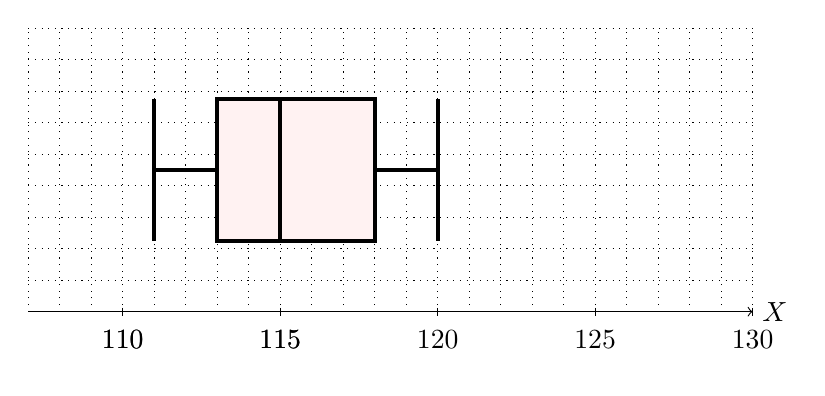
\begin{tikzpicture}[x=0.4cm,y=0.9cm]
         \draw[step=0.4cm,,dotted,color=black] (107,0) grid (130,4);
		\draw[->] (107,0) -- (130,0) node[right] {$X$} ;
		\foreach \X in {110,115,110,115,120,125,130} {
			\draw (\X,0.05cm) -- (\X,-0.05cm) node[below] {$\X\strut$};}
		\draw[ultra thick][fill=red!5] (113,1) rectangle (118,3);
  	\draw[ultra thick] (115,1) -- (115,3);

		\draw[ultra thick] (111,1) -- (111,3);
		\draw[ultra thick] (111,2) -- (113,2);
		\draw[ultra thick] (118,2) -- (120,2);
		%\draw[ultra thick] (4,1) -- (4,3);
		\draw[ultra thick] (120,1) -- (120,3);

			\end{tikzpicture}\\
	\end{center}

\begin{parts}
    


\part[3] Lequel des énoncés suivants est vrai?

  \begin{checkboxes}
\choice La médiane n'est pas au bon endroit.  %  X1
\choice Il devrait y avoir deux points: un à 105,5 et un à 125,5.
\choice La moustache de gauche devrait être à  105,5. 
\choice La moustache de droite devrait être à 125,5.
\choice Il n'y a aucune erreur.
\end{checkboxes}

\vspace{0.5cm}

\part[3] Pensez-vous que la loi normale modélise bien les données représentées? \textit{\textbf{Expliquez.}}

\vspace{4cm}

\end{parts}

\pageblanche

\question 

\begin{parts}
    \part[2] La corrélation de Spearman donne la même chose que la corrélation de Pearson.
    \begin{checkboxes}
        \choice Vrai
        \choice Faux
    \end{checkboxes}

    \vspace{0.25cm}

    \part[2] Si $X_1,...,X_n$ sont mesurés en $km$ la variance est en $km^2$ et l'écart-type est en $km$.
        \begin{checkboxes}
        \choice Vrai
        \choice Faux
    \end{checkboxes}

    \vspace{0.25cm}


    \part[2] Dans un échantillonnage probabiliste, il n'est pas nécessaire connaître la probabilité de sélection de tous les individus.
            \begin{checkboxes}
        \choice Vrai
        \choice Faux
    \end{checkboxes}

    \vspace{0.25cm}

    \part[2] La médiane est très sensible au valeurs extrêmes.
            \begin{checkboxes}
        \choice Vrai
        \choice Faux
    \end{checkboxes}

    \vspace{0.25cm}

        \part[2] Si je constate que les variables $X$ et $Y$ sont fortement corrélées, il est certain que $X$ cause $Y$ ou que $Y$ cause $X$.
            \begin{checkboxes}
        \choice Vrai
        \choice Faux
    \end{checkboxes}

    \vspace{0.25cm}
    
        \part[4] La non-réponse n'induit pas nécessairement un biais. \textit{\textbf{Expliquez.}}
            \begin{checkboxes}
        \choice Vrai
        \choice Faux
    \end{checkboxes}

    \vspace{3.25cm}

    \part[4] Une firme de sondage publie ce résultats: <<Notre enquête, menée au téléphone en utilisant comme base de sondage la liste des gens qui possèdent une ligne fixe, nous permet d'affirmer que l'âge moyen des québécois est de 57 ans.>> 
    Expliquez deux problèmes possibles de cette étude.
\end{parts}

\pageblanche

\question Soit le graphique suivant:

\begin{center}
    
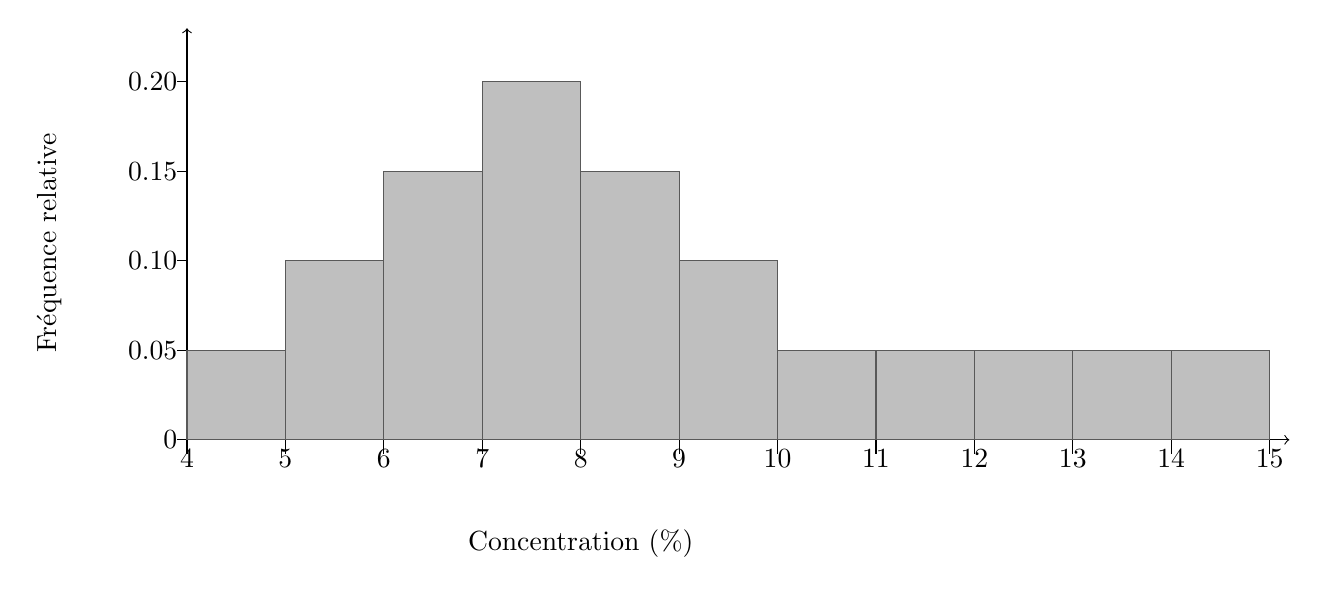
\begin{tikzpicture}[x=1.25cm, y=22.727cm] % 10 cm de large (8 unités) et 5 cm de haut (0.22 unités)
  % Axes
  \draw[->] (4,0) -- (15.2,0);
  \draw[->] (4,0) -- (4,0.23);

  % Graduations en x
  \foreach \x in {4,...,15} {
    \draw (\x,0) -- (\x,-0.008);
    \node[below] at (\x,0) {\x};
  }

  % Graduations en y
  \foreach \y/\lab in {0/0,0.05/0.05,0.10/0.10,0.15/0.15,0.20/0.20}{
    \draw (4,\y) -- (3.9,\y);
    \node[left] at (4,\y) {\lab};
  }

  % Titres d'axes
  \node[below] at (8,-0.045) {Concentration (\%)};
  \node[rotate=90] at (2.6,0.11) {Fréquence relative};

  % Barres : classes [4,5[, [5,6[, ..., [11,12[
  \foreach \x/\h in {4/0.05,5/0.1,6/0.15,7/0.20,8/0.15,9/0.1,10/0.05,11/0.05,12/0.05,13/0.05,14/0.05} {
    \fill[gray!50] (\x,0) rectangle (\x+1,\h);
    \draw[gray!70!black] (\x,0) rectangle (\x+1,\h);
  }
\end{tikzpicture}
\end{center}

\textit{Pour répondre aux questions suivantes, supposez qu'il n'y aucune observation sur les limites des classes et que les observations sont réparties de façon à peu près uniforme dans chaque classe.}

\begin{parts}
    \part[2] Comment se nomme cette représentation graphique?
    
    \vspace{2cm}

    \part[2] Si vous savez qu'il y a 36 observations pour lesquelles la concentration se trouve entre 4\% et 6\%, combien d'observations ont servi à produire ce graphique?

    \vspace{3cm}

    \part[2] Laquelle de ces deux mesures sera la plus grande?
    \begin{checkboxes}
        \choice La moyenne
        \choice La médiane
        \choice Il est impossible de le savoir
    \end{checkboxes}

    \vspace{0.25cm}

    \part[2] Quelle est la forme de cette distribution?
    \begin{checkboxes}
        \choice Symétrique
        \choice Asymétrique à droite
        \choice Asymétrique à gauche
    \end{checkboxes}
        \vspace{0.25cm}

    \part[4] Si on traçait un diagramme en boîte pour ces données, est-ce qu'il y aurait une/des valeur(s) aberrante(s)? \textit{\textbf{Expliquez.}}
\end{parts}

\pageblanche
\end{questions}

\end{document} 
